\documentclass{article}
\usepackage{amsfonts} % \mathbb
\usepackage[margin=0.5in]{geometry}
\usepackage[utf8]{inputenc}
\usepackage{graphicx}
\usepackage[backend=biber, style=apa]{biblatex}
\usepackage{amsmath}
\DeclareMathOperator{\sign}{sign}
\bibliography{bibli}

\title{Robust Digital Envelope Estimation Via Geometric Properties of an Arbitrary Signal}
\author{
  Carlos Tarjano
  \and 
  Valdecy Pereira
  }

\begin{document}

\maketitle

\begin{abstract} % 250 words

% estimate parameters from the signal itself
% broadband
% Dominant frequency as by-product
% we define several entities in the process, introducing a new measure of discrete curve curvature, hoping to consolidate the terminology in the area

  % background  
  Despite being an elusive concept, mathematically well defined only for artificially generated waves, the temporal amplitude envelope of a signal is essential for its complete characterization, being the primary information carrying medium in spoken voice and telecommunications, for example.
  intuitively, the temporal envelope can be understood as a smooth function on the same variable as the principal wave, or temporal fine structure, that modulates the signal, responsible for its outer shape. It is implied in this definition that the envelope is non periodic in general and is thus better addressed by specific techniques diverse from those used in the analysis of the periodic, rapidly changing wave it encompasses.
  % motivation
  Envelope detection techniques have applications in areas like health, sound classification and synthesis, seismology and speech recognition. Despite of that, a general approach to envelope detection of signals with rich spectral content seems to be lacking, and most methods involve manual intervention, like filter design, based on prior knowledge about the wave under investigation.
  % objective
  In this paper we propose a framework that uses intrinsic characteristics of a signal to estimate its envelope, eliminating the necessity of parameter tuning.
  % methods
  The approach here described draws inspiration from general, computational and differential geometry to isolate the frontier of an arbitrary signal. The concepts of alpha-shapes, concave hulls, arc-length parametrization and discrete curve curvature are adapted. We also define a pulse in the context of a arbitrary digital signal as a means to reduce dimensionality and the complexity of the proposed algorithm.
  % results
  
  % implications

\end{abstract}

{\bf Keywords:} DSP, alpha-shapes, envelope detection

\section{Introduction} % 500 words
% Opener sentence
Despite being ubiquitous in digital signal processing, the literature about envelope detection is very fragmented \parencite{2017LyonsDigital}. Besides, most envelope detection techniques are designed to account for very specific settings, like pure sinusoids with moderate noise contents, in line with the most common usages of those algorithms with artificial signals in the context of analog telecommunications.
% Literature review | Brief Context of Prior Research
In many natural signals, however, the temporal amplitude envelope of a signal plays a prominent role in the characteristics exhibited: According to \textcite{2017QiRelative}, for example, the envelope is at least as important as the fine structure of the soundwave in the context of the intelligibility of mandarin tones. That is also the case for English \parencite{1995ShannonSpeech}, where even envelopes modulating mostly noise were still capable of conveying meaning. The envelope helps to convey emotion and identity to the human voice \parencite{2018ZhuContributions}, and envelope preserving characteristics of concert halls are associated with their pleasantness \parencite{2011LokkiEngaging}.
% Cite current algorithms
When dealing with broadband signals, approaches tailored to specific applications are prevalent, such as the one presented by \textcite{2014YangFast} for the distributed monitoring of fibre optic or the one formulated by \textcite{2018AssefModeling} in the context of medical ultrasound imaging.

If one adresses the different units in the horizontal and vertical axes, one can transform the DSP problem of envelope detection in the geometric problem of defining the shape of a set of points in $ \mathbb{R}^2 $. For that purpose \textcite{1983Edelsbrunnershape} introduced the concept of alpha-shapes, a mathematically well defined extension to the convex hull of a finite set of points, related to the Delaunay triangulation and Voronoi diagrams of those points.

This approach is used in areas such as the detection of features in images \parencite{2016VarytimidisAlpha}, reconstruction of surfaces from a cloud of points \parencite{2015WuAutomated} and Spectroscopy \parencite{2019XuModeling}, with the last work, that involves the estimation and removal of the Blaze function -a kind of envelope- of a echelle spectrograph, being particularly align with what is intended here.

% Restate Your Question as Something Not Known or Fully Understood by Prior Research
Thus, in this paper we formulate a general approach to envelope detection, exploiting the intrinsic characteristics of a generic, spectrally complex, wave in order to avoid the need to manual intervention or parameter tuning.
% State the Significance of Your Question
While the robustness of the proposed approach allows it to be used as a plug in replacement for many methods encountered in the literature, we feel that it would be particularly useful for sound synthesis. 
The envelope is shown to add complexity to the spectral representation of a wave \parencite{2019TarjanoNeuro}, and a accurate description of the envelope would be useful for a cleaner spectral analysis. Moreover, the algorithm naturally divides a signal in pseudo-cycles, that could serve pragmatic building blocks for the reconstruction of the fine structure of the wave.
% State Your Claim | Objective | Hypothesis
In the context of sound synthesis, one would be able to apply specific methods for the recreation of the envelope, more in line with its smooth, slow varying and non periodic nature and a different approach to the periodic and relatively fast changes of the temporal fine structure.
% brief outlook on the structure of the paper


\section{Methodology} % 1000 words

% Essential background information
We start by defining a pulse as a series of consecutive samples in a discrete wave with the same sign. More formally, let $ W[i] \in \mathbb{R} \forall i \in \mathbb{N}_0, i < n \in \mathbb{N}_0 $ be a real, discrete and finite signal indexed, without loss of generality, over a subset of the natural numbers. This definition relates closely to the concept of an array or vector in programming languages, and is used in the interest of simplicity. A pulse $ P[j], j \in \mathbb{N}_0 $ in $ W $ can then be defined as a sequence of samples indexed by $ i $ such that $ \sign(W[a-1]) \ne \sign(W[a]) = \sign(W[a+1]) = \dots = \sign(W[b-1]) = \sign(W[b]) \ne \sign(W[b+1]) \forall a \le i \le b | a,b \in \mathbb{N}_0 $. In other words a pulse is a cluster of samples between the changes of sign in the original wave. For a continuous function, that would correspond to the pieces between it's roots, and would be equal to half the cycle of a sinusoid. Thus, in our analogy, two consecutive, opposed pulses have the potential do delimitate a pseudo-cycle, as illustrated in figure \ref{fig:pulses}. For that to be true, however, the pulses need to make part of the frontier, as will be defined later.

  \begin{figure}[h!]
    \centering
      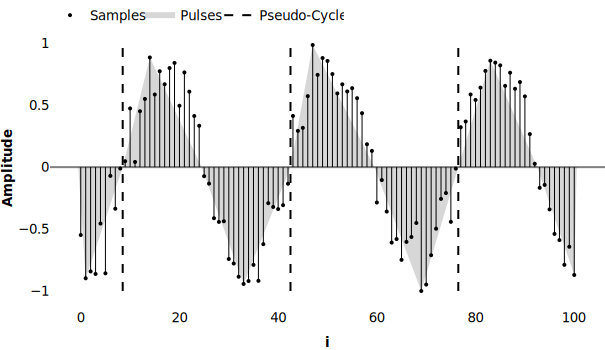
\includegraphics[width=0.8\linewidth]{01Pulses.pdf}
    \caption{The grey areas encompass the simplified convex hulls of the pulses. The dashed lines mark the frontier between pseudo-cycles}
    \label{fig:pulses}
  \end{figure}

As we are seeking a geometric treatment of the subject, it is first necessary to make abscissa and ordinate units consistent. this can be accomplished by multiplying each sample of the signal by the average length of the pulses, after having divided by the average of signal amplitudes, putting both axes in the same frame related unit $i$, that relates to time by the equation $i = t \ \mathit{fps}$. One can call this approach arc length regularization, as it translates the widespread approach of arc length parametrization to a non parametric setting.

% Define envelope

It will be useful to introduce the concept of a frontier as the set of points $ (i, W[i]) $ that are closest to the unknown smooth, continuous envelope of the signal. Because we are interested in a function that is smooth over the whole domain of the wave, we can assume that, in the scale of a pulse, this function will be very close to a horizontal straight line and, thus, won't touch any point inside the convex hull defined by the pulse. By the same token, as the change in amplitude from one pulse to the next is motivated by changes in the temporal envelope, one can assume that $ \max(P[j]) \approx \max(P[j+1]) $ and approximate the convex hull of a pulse with the rectangle whose length is defined by the points where the pulse crosses the horizontal axis and whose height is equal to the point of max amplitude; this will allow a considerable dimension reduction as this rectangular pulse becomes the atomic unit for the rest of the method.

Besides, those definitions will allow us to derive the frontier of a wave using an alpha-shapes inspired algorithm without the need to compute the Delaunay triangulation first. Translating the intuitive explanation of alpha-shapes in \textcite{1994EdelsbrunnerThree}, we can say that the points in the frontier are those touched by a circle outside the signal that is not allowed to contain any point of the signal; one can picture a circle being rolled above (or below, in the case of the negative envelope) the signal, and marking the points it touches as frontier points.

% snowball image

It is now necessary to infer the appropriate radius of such a circle and, to that end, a measure of the instantaneous curvature of a discrete function is needed. Discrete curvature estimation is an important task in image processing \parencite{2010FleischmannNovel} for which no default definition exists; The two possible approaches are the derivation of direct methods that use characteristics of the discrete wave to calculate its curvature at each point, or the calculation of the curvature of a curve fitted to the discrete wave \parencite{2001CoeurjollyDiscrete}. 
To fit a polynomial to the a generic wave two approaches are readily available: the least mean squares approach, that seeks to minimize the dependant variable errors and the total least squares problem, that treat both variables symmetrically \parencite{1980GolubAnalysis}.
The geometric, symmetrical nature of the problem excludes the more computationally economic least mean squares approach however, leaving us with the total least squares, for which no general closed form solutions are available \parencite{2007MarkovskyOverview}; this leads us to turn our attention to direct approaches of curvature estimation.

\subsection{Discrete Curvature Estimation - The Equivalent Circle Approach}

As previously stated, no default discrete curvature definition exists

% osculating circle image, fitted line

% For a continuous, twice differentiable function $ y = f(x); x, y \in \mathbb{R} $, the curvature as a function of the independent variable is given by $ \kappa(x) = \frac{f''(x)}{(f'(x)^2 + 1)^{\frac{3}{2}}} $ which is also the inverse of the radius of the osculating circle tangent to the curve at $ x $. Since we are assuming smoothness of envelope in the neighbourhood of a pulse, it makes sense to approximate it with a parabola $ y(x)=ax^2+bx+c $, since a higher order polynomial would provide unnecessary complexity. Besides some characteristics of the parabola derived from its relation with Bezier curves will be useful later.

% Therefore, the definition of the curvature becomes $ \kappa(x) = \frac{2 a}{\big( (b + 2 a x)^2 + 1 \big)^\frac{3}{2}} $ with the average curvature between points $ x_0 $ and $ x_1 $ given by equation \ref{eq:1}.

% \begin{equation} \label{eq:1}
%   \overline{\kappa}(x) = 
%   \frac{
%       \left( \dfrac{2 a x_1 + b}{\sqrt{\big(2 a x_1 + b \big)^2+1}} - \dfrac{2 a x_0 + b}{\sqrt{\big(2 a x_0 + b \big)^2+1}} \right) 
%   }{
%     (x_1 - x_0)
%   }
% \end{equation}

% \subsection{Theory}


  
\section{Results}

\section{Discussion + Conclusion}

\section{References}
\printbibliography[heading=none]

\end{document}
